\documentclass[10pt]{beamer}

\usepackage[utf8]{inputenc}
\usepackage[T1]{fontenc}
\usepackage[french]{babel}
\usepackage[ddmmyyyy]{datetime}
\usepackage{listings,lstautogobble,graphicx,tikz}
\usepackage{lmodern}
\usetikzlibrary{arrows,automata}
\usetikzlibrary{positioning}

\usetheme{Warsaw}
\useinnertheme{rectangles}
\setbeamerfont{headline}{size=\large}
\setbeamerfont{frametitle}{size=\normalsize}

%Plan/Sommaire automatique avant chaque section
\AtBeginSection[]{
  \begin{frame}
  \frametitle{Plan}
  \tableofcontents[currentsection]
  \end{frame}
}

\author{Jean-Didier Pailleux - Robin Feron - Romain Robert - Damien Thenot - Maxence Joulin}
\institute{UVSQ}
\date{\today}
\usepackage{../tex/myInfolines}
\usepackage{longtable,array}
\title{Test de Primalité}

\begin{document}
	\begin{frame}
		\titlepage
	\end{frame}
	
	\section*{Introduction}
        \begin{frame}
            \begin{itemize}
            \item \textbf{Nombre Premier:} Entier divisible par 1 et lui-même.\\pause
            \vspace{1em}            
            \item \textbf{Test Probabiliste :} Test avec marge d'erreur très faible mais rapide.  \\
            \vspace{1em}
            \item \textbf{ Test Deterministe :} Test fiable mais plus lent.    \\
            \vspace{1em}
            \item \textbf{$2^{64}$ :} Taille maximale des nombre a tester => Unsigned long long int  \\
            \vspace{1em}
            \item \textbf{Nombre Hautement Composé :} Entier qui possède strictement plus de diviseur que les nombres qui le précède\\
            \end{itemize}            
        \end{frame}
	
	\begin{frame}
		\tableofcontents
	\end{frame}
	
	\section{Etat de l'art}
\begin{frame}{Les tests de primalit\'e d\'eterministes}
\begin{block}{Les m\'ethodes na\"ives}
 \begin{itemize}
 \item {
   Le Crible d'Eratosth\`ene: efficace mais co\^uteux en terme de m\'emoire (Memory Bound)
 }
 \item {  
   Les divisions euclidienne et PGCD: simples mais coute\^uses en calculs (Computation Bound)
 }
 \end{itemize}
\end{block} \pause

\begin{block}{Les m\'ethodes modernes}
 \begin{itemize}
 \item {
   Pocklington: Factorisation partielle en nombres premiers
 }
 \item {
   AKS: R\'esolution d'inconnues selon le petit th\'eor\`eme de Fermat: complexit\'e polynomiale tr\`es interressante pour les grands nombres
 }
 \end{itemize}
\end{block}
\end{frame}

\begin{frame}{Un test de primalit\'e probabiliste et Nombres hautement compos\'es}
\begin{block}{Miller Rabin}
 Utilisation du petit th\'eor\`eme de Fermat: \\ $a^p-1 \equiv 1 \pmod p$.\\
 Ne permet que d'affirmer qu'un nombre est probablement premier. Un nombre d'iteration suffisant peut permettre d'atteindre des taux d'erreurs infimes pour un temps de calcul tr\`es faible.
\end{block} \pause

\begin{block}{Les nombres hautement compos\'es}
 \begin{itemize}
 \item {
   M\'ethode naive: Chercher le nombre de diviseurs de tout les nombres inferieurs à N
 }
 \item {
   M\'ethode utilisant une propri\'et\'e de leur forme: une d\'ecomposition en nombres premiers à facteurs d\'ecroissants.
 }
 \end{itemize}
\end{block}
\end{frame}

	\section{Implémentation}
		\begin{frame}
		\begin{block}{Langages de programmation } 
		\begin{itemize}
		\item Le langage C++ : langage adapté pour la programmation procédurale et orientée objet +  bibliothèques pour les grands entiers supérieur , chronométrer et autre.\\
		\item Le langage Shell : enchaînement de commandes pour les tests.
		\end{itemize} \pause
		\vspace{2em}		
		\end{block}
		
		\begin{block}{Outils}
		\begin{itemize}
			\item La bibliothèque GMP : manipulation de nombres supérieur à $2^{64}$.
			\item La bibliothèque NTL : fonctions pour l'arithmétique modulaire disponible.
			\item CMkake : pour la compilation du projet.
			\item Github : dépôt du projet + travail collaboratif.
		\end{itemize}
		\end{block}
		\end{frame}
	\section{Analyse des Résultats}
		\begin{frame}
		\textbf{Lancement d'une phase de test :}

	\begin{itemize}
		\item Appel d'un script bash ou lancement en ligne de commande.\\
		\item Script bash => test sur un fichier ou plage de valeurs ou test normal.
		\begin{block}{Options}\vspace{-1em}
	\begin{center}\footnotesize\begin{longtable}{l l}		
	\textbf{a} : Tous les algorithmes  & \textbf{k} : AKS\\
	\textbf{e} : Euclide (computation bound) & \textbf{o} : Modulo (computation bound)\\
	\textbf{m} : Crible d'eratosthene & \textbf{p} : Pocklington\\
	\textbf{i} : Miller-Rabin & \textbf{h} : Nombre hautement composé naive\\
	\textbf{H} : Nombre hautement composé def\\
	\end{longtable}\end{center}
	\end{block}
		\item Lequel utiliser ?\\
		\item Itération ?\\
		\item Combien de nombre ?\\
		\item Donner les nombres\\
	\end{itemize}
\end{frame}

\begin{frame}
\begin{figure}[!ht]	
		\begin{center}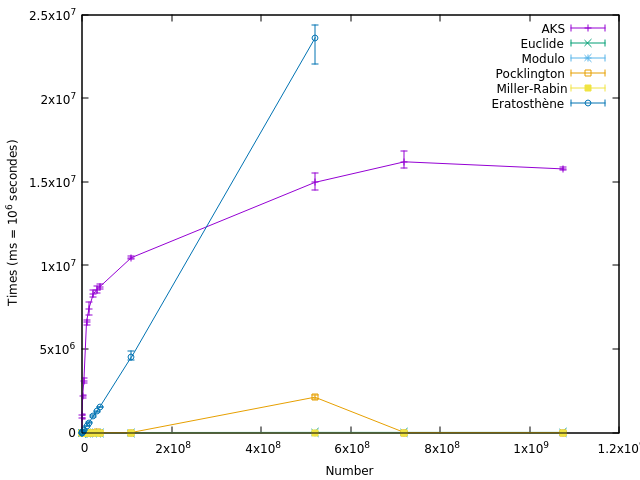
\includegraphics[scale=0.55]{result.png}\end{center}
		\caption{Évolution du temps d'exécution pour les 6 tests de primalité (AKS, Pocklington, Miller-Rabin, Euclide, Ératosthène et Modulo). }
		\label{fg:fig1}
\end{figure}
\end{frame}

\begin{frame}
\begin{figure}[!ht]	
		\begin{center}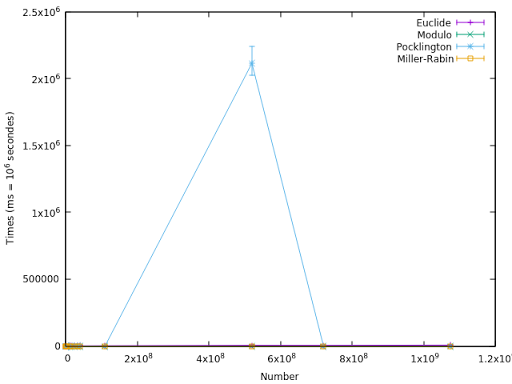
\includegraphics[scale=0.5]{Zoom1.png}\end{center}
		\caption{Zoom de la figure \ref{fg:fig1} sur (Pocklington, Miller-Rabin, Euclide et Modulo).}
		\label{fg:fig2}
\end{figure}
\end{frame}
		
\begin{frame}
\begin{figure}[!ht]	
		\begin{center}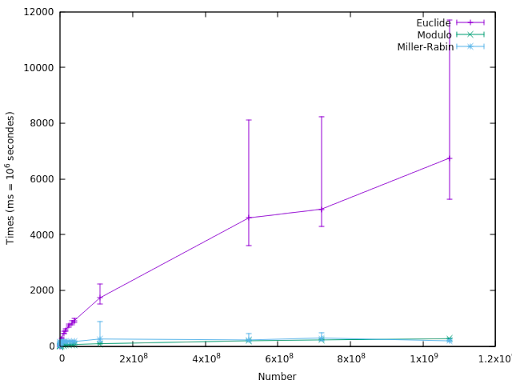
\includegraphics[scale=0.5]{Zoom2.png}\end{center}
		\caption{Zoom de la figure \ref{fg:fig1} sur (Miller-Rabin, Euclide et Modulo).}
		\label{fg:fig3}
\end{figure}
\end{frame}

\begin{frame}
	\begin{figure}[!ht]	
		\begin{center}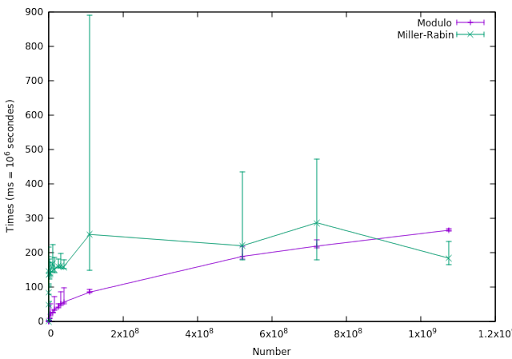
\includegraphics[scale=0.5]{Zoom3.png}\end{center}
		\caption{Zoom de la figure \ref{fg:fig1} sur (Miller-Rabin et Modulo).}
		\label{fg:fig4}
	\end{figure}
\end{frame}
	
		\begin{frame}
		\color{blue} Figures - \color{black}\textit{Évolution du temps d'exécution pour les 6 tests de primalité sur une plage de données}
		
		\footnotesize\begin{longtable}{l r}		
	\hspace{-2em} 
 		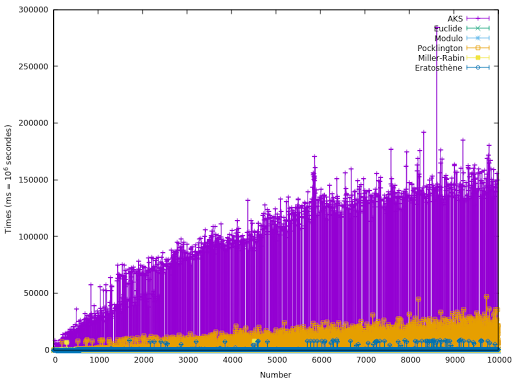
\includegraphics[scale=0.3]{RANGE.png}  & 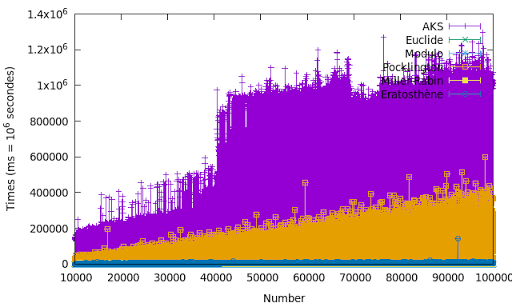
\includegraphics[scale=0.3]{RANGE2.png}\\
		 \textit{Plage $[1:10 000]$} & \textit{Plage $[10 000:100 000]$} \\
		 100\% de réussite pour Miller-Rabin &  100\% de réussite pour Miller-Rabin\\
	\end{longtable}
		\end{frame}

	\section{Bilan Technique}
		\begin{frame}
			\begin{itemize}
			\item \textbf{Eratosthène:} Création d'un tableau de taille N+1 dans le crible => limité au niveau de la RAM pour N grand sur nos machines. Complexité de N pour le remplissage de la liste memory\_bound. \\
			\vspace{1em}			
			\item \textbf{Euclide:} Effectue $\sqrt{2^{log_2(n)}}$ divisions euclidiennes => Exécution en temps exponentiel\\
			\vspace{1em}
			\item \textbf{Pocklington:} Limite causé par la factorisation du nombre N-1 => factorisation très longues pour N très grand.\\
			\vspace{1em}
			\item \textbf{Miller-Rabin:} Résultats faux dans certains cas + Nombre d'itérations demandé élevé pour un meilleur résultat => augmentation du temps d'exécution.  \\
			\vspace{1em}
			\item \textbf{AKS:} \underline{Avantage:} Sa complexité en $log(n)^{12}$.\\
						\underline{Inconvénient:} Utilisation de NTL qui effectue des vérifications superflue + Implémentation compliquée.\\
			
			\end{itemize}	
			\end{frame}
		
		

	\section{Conclusion}
		\begin{frame}
	\begin{itemize}
        \item De grands temps de calculs pour les tests déterministes. \vspace{1em}
        \item Méthodes naïves efficaces pour les petits nombres. \vspace{1em}
        \item Tests probabiliste une bonne idée? \vspace{1em}
        \item \textbf{Possibilités de parallélisation :} Une ouverture sur des techniques de calcul en parallèle pourrait être appliqués.
     \end{itemize}
		\end{frame}	
		
		\section*{Organisation interne du groupe}
	\begin{frame}
\textbf{Tableau de répartition du travail:} \\
	
	\begin{center}\vspace{-1em}\footnotesize\begin{longtable}{|>{\centering}m{3.0cm}|>{\centering}m{1.5cm}|>{\centering}m{1.2cm}|>{\centering}m{1.2cm}|>{\centering}m{1.2cm}|>{\centering\arraybackslash}m{1.2cm}|}			
		\hline \multicolumn{1}{|c|}{\textbf{Tâches}} & \multicolumn{1}{c|}{\textbf{Jean-Didier}} & \multicolumn{1}{ c|}{\textbf{Maxence}} & \multicolumn{1}{ c|}{\textbf{Romain}} & \multicolumn{1}{ c|}{\textbf{Robin}} & \multicolumn{1}{c|}{\textbf{Damien}}\\
		\hline 	Eratosthène/Memory Bound & x & ~ & ~ & ~ & ~ \\
		\hline 	Euclide/Computation Bound & ~ & x & ~ & ~ & ~ \\
		\hline 	AKS & ~ & ~ & x & ~ & ~ \\
		\hline 	Pocklington & ~ & ~ & ~ & ~ & x \\
		\hline 	Miller-Rabin & ~ & ~ & ~ & x & ~ \\
		\hline 	Highly Composite & x & ~ & ~ & ~ & ~ \\
		\hline 	Cmake  & x & x & ~ & ~ & ~ \\
		\hline  Script/main & x & x & ~ & ~ & ~ \\
		\hline
	\end{longtable}\vspace{-2.2em}\end{center}
	\end{frame}
\end{document}
